\documentclass[conference]{IEEEtran}
\IEEEoverridecommandlockouts
% The preceding line is only needed to identify funding in the first footnote. If that is unneeded, please comment it out.
\usepackage{cite}
\usepackage{amsmath,amssymb,amsfonts}
\usepackage{algorithmic}
\usepackage{graphicx}
\usepackage{textcomp}
\usepackage{xcolor}
\usepackage{tabularx}
\usepackage{multirow}
\usepackage{graphics} % for pdf, bitmapped graphics files
\usepackage{subfig}
\usepackage{subcaption}
\usepackage{hyperref}
\usepackage{academicons}
\usepackage{xcolor}
\usepackage{listings}
\usepackage{tabularx} % Asegúrate de incluir este paquete

\usepackage{tikz}
\usetikzlibrary{shapes.geometric, arrows}

\usetikzlibrary{shapes.geometric, arrows}

\tikzstyle{startstop} = [rectangle, rounded corners, minimum width=3cm, minimum height=1cm,text centered, draw=black, fill=red!30]
\tikzstyle{process} = [rectangle, minimum width=3cm, minimum height=1cm, text centered, draw=black, fill=blue!30]
\tikzstyle{arrow} = [thick,->,>=stealth]


\def\BibTeX{{\rm B\kern-.05em{\sc i\kern-.025em b}\kern-.08em
		T\kern-.1667em\lower.7ex\hbox{E}\kern-.125emX}}

% Color Enlace
\definecolor{colorEnlace}{RGB}{0, 0, 0}
\hypersetup{
	colorlinks=true,
	linkcolor=colorEnlace,
	citecolor=colorEnlace,
	urlcolor=colorEnlace,
	pdfauthor={Davis Bremdow Salazar Roa},
	pdftitle={Sistemas Embebidos}
}
\definecolor{mybg}{rgb}{0.97,0.97,0.97}
\definecolor{mygray}{gray}{0.4}
\definecolor{mygreen}{rgb}{0,0.6,0}
\definecolor{myblue}{rgb}{0,0,0.8}
\definecolor{mypurple}{rgb}{0.58,0,0.82}
\definecolor{myred}{rgb}{0.7,0,0}

\lstdefinelanguage{MatlabEnhanced}{
	language=Matlab,
	morekeywords={[2]linspace,plot,title,xlabel,ylabel,legend,grid},
	morekeywords={[3]sin,cos,exp,log,sqrt},
	keywordstyle=\color{myblue}\bfseries,
	keywordstyle=[2]\color{mypurple},
	keywordstyle=[3]\color{myred},
	commentstyle=\color{mygreen}\itshape,
	stringstyle=\color{mygray},
	morecomment=[l]%
}

\lstset{
	language=MatlabEnhanced,
	backgroundcolor=\color{mybg},
	frame=single,
	basicstyle=\ttfamily\small,
	showstringspaces=false,
	numbers=none,              %
	xleftmargin=0pt,           %
	framexleftmargin=0pt,      
	framexrightmargin=0pt,
	framextopmargin=2pt,
	framexbottommargin=2pt,
	breaklines=true,
	tabsize=1,
}

% Control 
\usepackage{amsmath}
\begin{document}
	
	\title{Circuito de radiofrecuencia - modulador AM}
	\author{
		\makebox[\textwidth][c]{\large\textbf{Universidad Nacional de San Antonio Abad del Cusco}}\\
		\makebox[\textwidth][c]{\normalsize\textit{Escuela profesional de Ingeniería Electrónica}}\\
		\makebox[\textwidth][c]{\normalsize\textit{Telecomunicaciones I}}\\
		\and
		\IEEEauthorblockN{Ing. Milton Velasquez Curo}
		\IEEEauthorblockA{Ingeniero Electrónico \\
			Cusco, Perú \\
			milton.velasquez@unsaac.edu.pe}
		\and
		\IEEEauthorblockN{Davis Bremdow Salazar Roa - 200353}
		\IEEEauthorblockA{Estudiante de Ingeniería Electrónica \\
			Cusco, Perú \\
			200353@unsaac.edu.pe}
	}
	
	\maketitle
	\begin{abstract}
		Los circuitos de radiofrecuencia (RF) en modulación en amplitud (AM) son fundamentales en los sistemas de comunicación analógica, ya que permiten la transmisión y recepción de señales de audio mediante ondas electromagnéticas. Su importancia radica en su simplicidad, bajo costo y amplia cobertura, lo que los hace útiles en aplicaciones como la radiodifusión, sistemas de emergencia y transmisiones a larga distancia.
	\end{abstract}
	
	\begin{IEEEkeywords}
		modulación en amplitud, frecuencia portadora, demodulación AM, oscilador RF, amplificador de señal, antena transmisora, receptor superheterodino, filtro sintonizado, ancho de banda, comunicación analógica.
	\end{IEEEkeywords}
	
	%% Contenido del documento
	\section{Amplificador de Radiofrecuencia}
	
	En la figura \ref{fig:circuito-modulador} se puede apreciar un circuito didáctico para la generación de señales de radiofrecuencia en el ámbito de la propagación AM, siendo un amplificador del tipo A debido a la topologia del circuito en emisor común y el acoplo inductivo, capacitivo en la salida del mismo y el cual se define en \cite{boylestad2010}.
	
	Siendo además en esta etapa de amplificación (entrada) en la cual se realiza el mezclado de las señales portadora y moduladora.
	
	Estando este circuito compuesto por 2 etapas de amplificación una definida en la etapa de modulación mediante el empleo del transistor $Q_1$ y la segunda en la etapa de salida (demodulación) mediante el amplificador operacional $LM324ANG$ configurado como no inversor.
	
	Además de forma general este circuito esta compuesto por el circuito mezclador definido por el transistor $Q_1$, el acoplo capacitivo previo a la etapa del detector de envolvente y la amplificación de la señal demodulada que se aprecia en la parte final del circuito mediante el OPAM.
	
	\section{Señales en el circuito de Radiofrecuencia}
	
	En el circuito de radiofrecuencia se definieron 4 puntos de observación ubicados en puntos estratégicos para la observación de las señales entre las cuales destacan:
	
	\begin{enumerate}
		\item Portadora
		\item Señal de información (Moduladora)
		\item Señal modulada
		\item Señal demodulada
	\end{enumerate}
	
	Siendo las mismas representadas por los colores celeste, rojo, verde y azul respectivamente como se aprecia en la figura \ref{fig:circuito-modulador} 
	
	\begin{figure}[h]
		\centering
		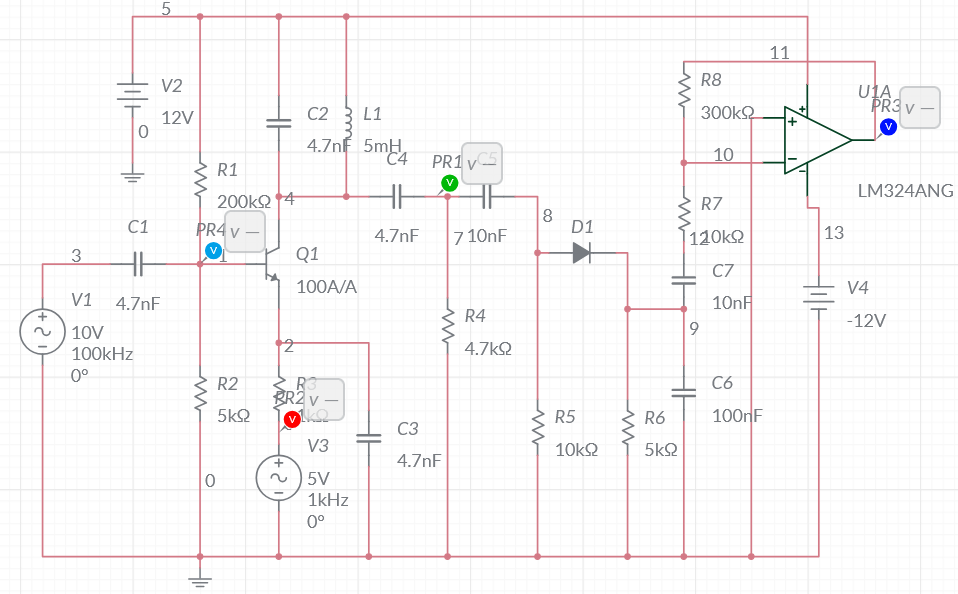
\includegraphics[width=0.5\textwidth]{media/circuito-modulador}
		\caption{Circuito modulador y demodulador de Radio Frecuencia}
		\label{fig:circuito-modulador}
	\end{figure}
	
	Las señales de salida de forma general se muestran en la figura \ref{fig:seniales-etapa} en las cuales también se guarda la relación de colores descritas anteriormente.
	
	\begin{figure}[h]
		\centering
		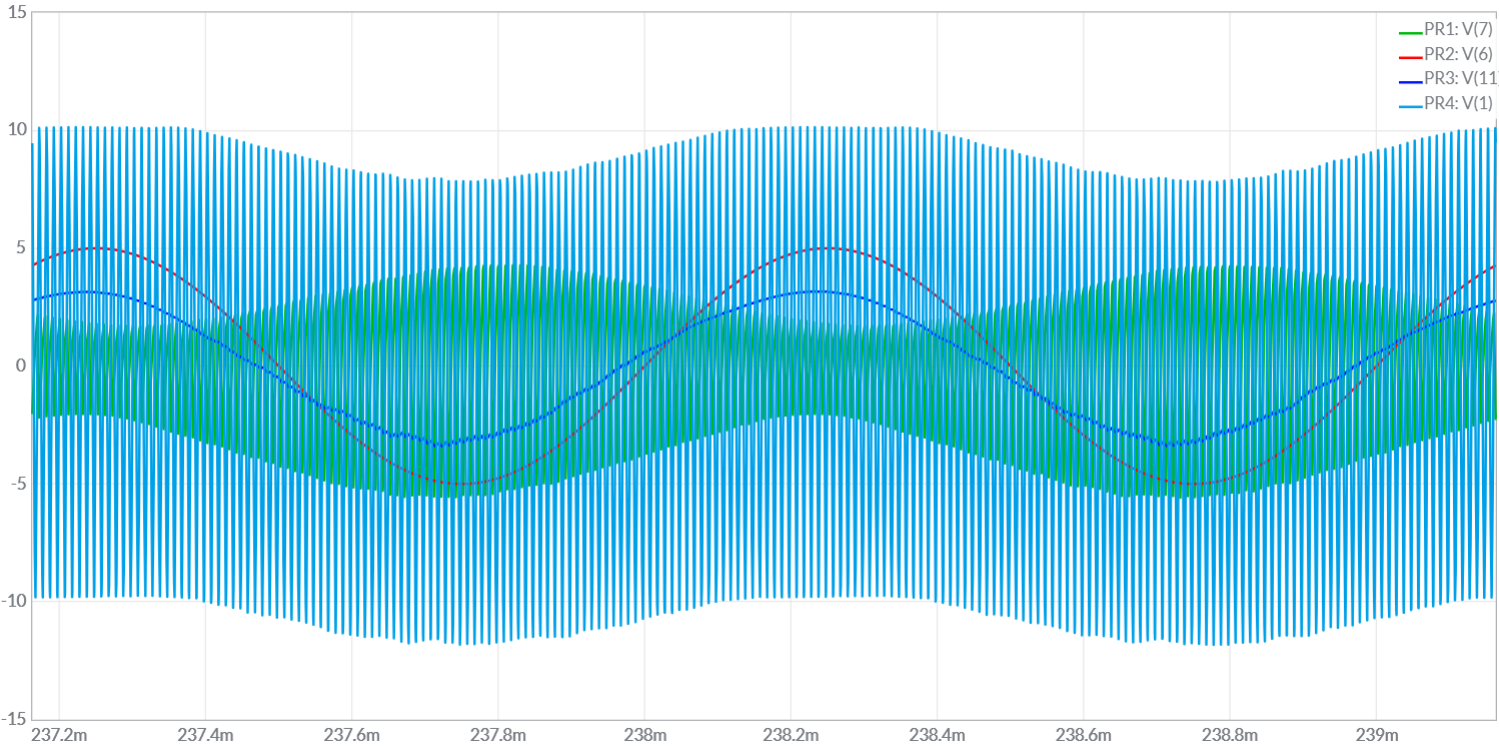
\includegraphics[width=0.5\textwidth]{media/seniales-etapa}
		\caption{Panorama general de las señales de salida}
		\label{fig:seniales-etapa}
	\end{figure}
	
	No obstante de forma individual cada forma de onda también se puede usar para establecer o identificar el tipo de señal en función a su frecuencias y características de las mismas, por ejemplo en la señal de la figura \ref{fig:senial-moduladora} se puede apreciar una onda de baja frecuencia a simple vista lo cual se puede comprobar mediante el cálculo del periodo o frecuencia.
	
	\begin{align*}
		T_2 &= 238.25ms\\ 
		T_1 &= 237.25ms \\
		P  &= T_2 - T_1 \\
		P &= 1ms\\
		F &= 1000 Hz
	\end{align*}
	
	La frecuencia resultante equivalente a $1000 Hz$ aunque no despreciable cataloga esta señal como una de baja frecuencia en comparación a la señal portadora de $100K Hz$.
	
	\begin{align*}
		T_2 &= 277.21ms\\ 
		T_1 &= 277.20ms \\
		P  &= T_2 - T_1 \\
		P &= 1us\\
		F &= 100k Hz
	\end{align*}
	
	\begin{figure}[h]
		\centering
		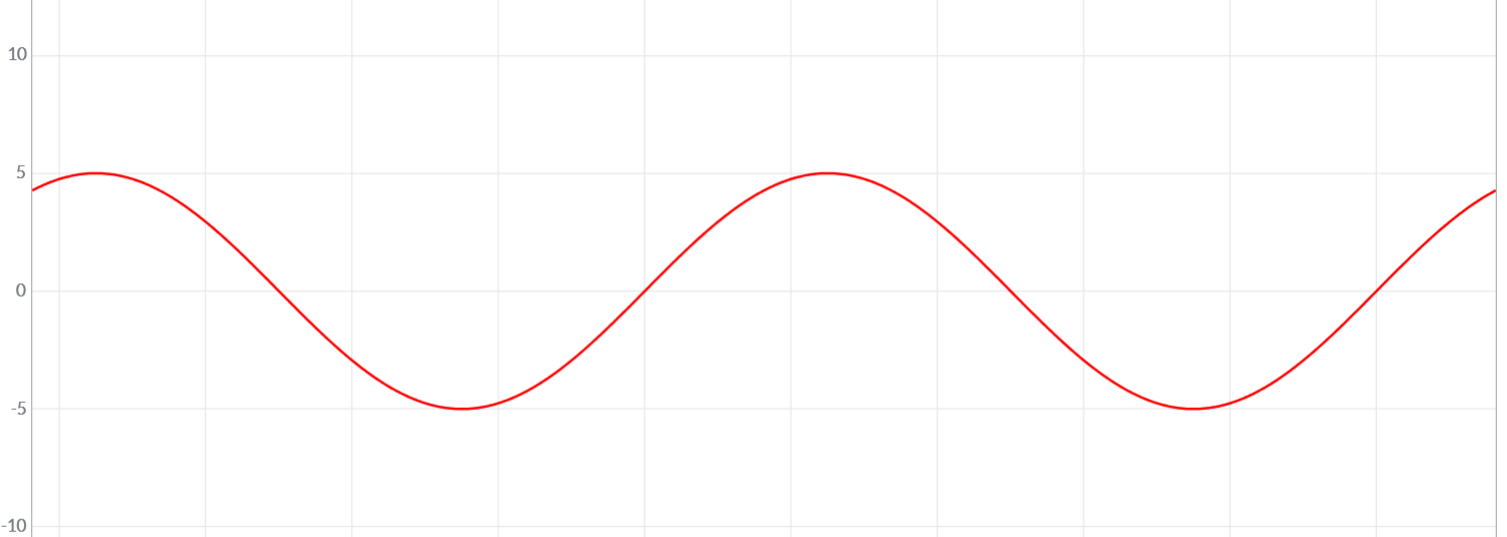
\includegraphics[width=0.5\textwidth]{media/senial-moduladora}
		\caption{Señal moduladora}
		\label{fig:senial-moduladora}
	\end{figure}
	
	
	\section{Tipo de Modulación}
	
	Para la determinar del tipo de modulación se analizo en primera instancia la forma de onda de la señal modulada mostrada en la figura \ref{fig:senial-modulada} en la cual se puede observar un offset la cual eleva la señal hasta 4.256 [V] lo cual indica la influencia de la portadora en la señal modulada resultante.
	
	\begin{figure}[h]
		\centering
		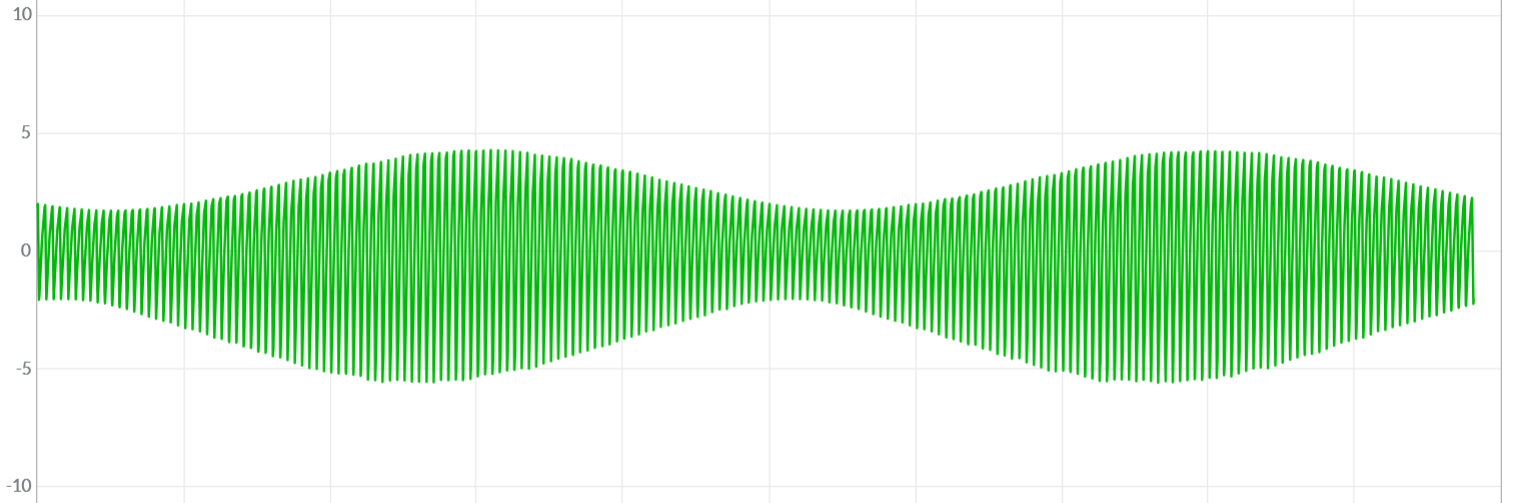
\includegraphics[width=0.5\textwidth]{media/senial-modulada}
		\caption{Señal modulada DSB - LC}
		\label{fig:senial-modulada}
	\end{figure}
	
	En adición también se pudo apreciar en la etapa de demodulación el empleo de un diodo y una red paralelo de un resistor y capacitor que se muestra en la figura \ref{fig:detector-envolvente}, las cuales son empleadas comúnmente para la recuperación de información en la modulación AM o $DSB - LC$ a causa de su facilidad como se define en \cite{stremler2006}
	
	\begin{figure}[h]
		\centering
		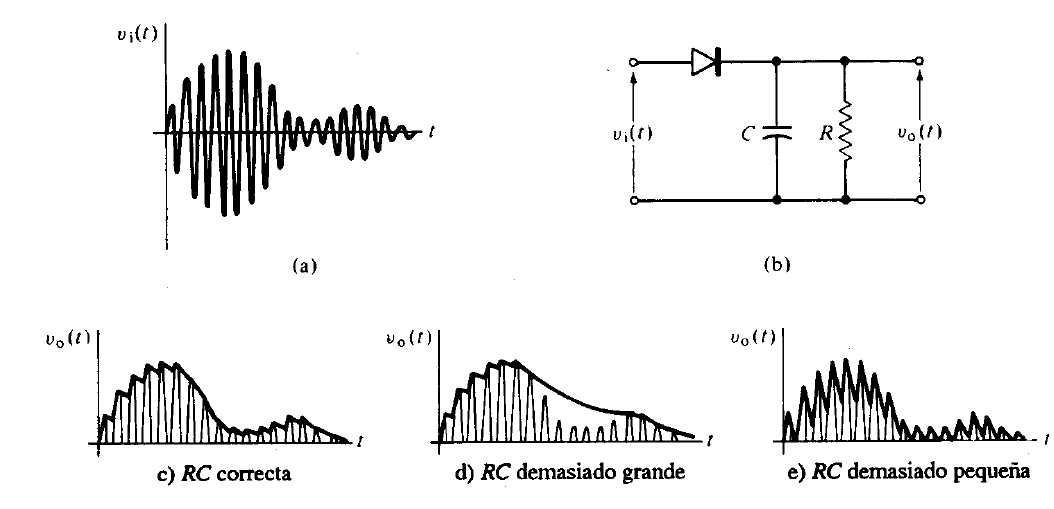
\includegraphics[width=0.5\textwidth]{media/detector-envolvente}
		\caption{Circuito detector de envolvente}
		\label{fig:detector-envolvente}
	\end{figure}
	
	
	\section{Observaciones}
	
	Finalmente en el circuito de la figura \ref{fig:circuito-modulador} la señal portadora es generada mediante el empleo de una fuente de voltaje de $10 V$ a una frecuencia de $100 Hz$, empero este tipo de señales generalmente es generada mediante el empleo de circuitos osciladores Colpitts o Harley como se define en \cite{tomasi_comunicaciones}, siendo su esquema circuital el que se muestra en la figura \ref{fig:oscilador-colpitts}
	
	\begin{figure}[h]
		\centering
		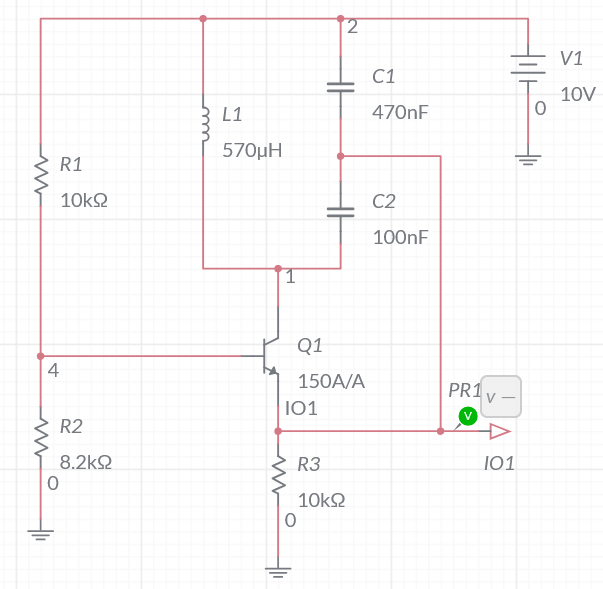
\includegraphics[width=0.5\textwidth]{media/oscilador-colpitts}
		\caption{Circuito oscilador Colpitts}
		\label{fig:oscilador-colpitts}
	\end{figure}
	
	Por otro lado para la etapa de mezclado se hace uso de la no linealidad del amplificador transistorizado al aplicar la señal moduladora en el emisor variando la ganancia del amplificador en función a la envolvente de esta señal, obteniendo como salida la señal de la figura \ref{fig:senial-modulada} o señal modulada.
	
	Un circuito referencia para este proceso se define en \cite{tomasi_comunicaciones} y se muestra en la figura \ref{fig:circuito-modulante-tomasi}. 
	
	\newpage
	
	\begin{figure}[h]
		\centering
		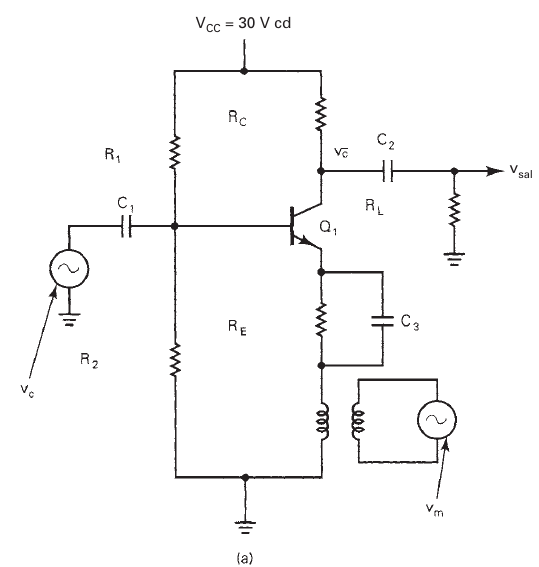
\includegraphics[width=0.5\textwidth]{media/circuito-modulante-tomasi}
		\caption{Circuito de modulación AM con acoplo de emisor}
		\label{fig:circuito-modulante-tomasi}
	\end{figure}
	
	
	\bibliographystyle{IEEEtran}
	\bibliography{biblio}
\end{document}






















